%%
%% This is file `example.tex',
%% generated with the docstrip utility.
%%
%% The original source files were:
%%
%% coppe.dtx  (with options: `example')
%% 
%% This is a sample monograph which illustrates the use of `coppe' document
%% class and `coppe-unsrt' BibTeX style.
%% 
%% \CheckSum{1648}
%% \CharacterTable
%%  {Upper-case    \A\B\C\D\E\F\G\H\I\J\K\L\M\N\O\P\Q\R\S\T\U\V\W\X\Y\Z
%%   Lower-case    \a\b\c\d\e\f\g\h\i\j\k\l\m\n\o\p\q\r\s\t\u\v\w\x\y\z
%%   Digits        \0\1\2\3\4\5\6\7\8\9
%%   Exclamation   \!     Double quote  \"     Hash (number) \#
%%   Dollar        \$     Percent       \%     Ampersand     \&
%%   Acute accent  \'     Left paren    \(     Right paren   \)
%%   Asterisk      \*     Plus          \+     Comma         \,
%%   Minus         \-     Point         \.     Solidus       \/
%%   Colon         \:     Semicolon     \;     Less than     \<
%%   Equals        \=     Greater than  \>     Question mark \?
%%   Commercial at \@     Left bracket  \[     Backslash     \\
%%   Right bracket \]     Circumflex    \^     Underscore    \_
%%   Grave accent  \`     Left brace    \{     Vertical bar  \|
%%   Right brace   \}     Tilde         \~}
%%
\documentclass[dsc]{coppe}

\usepackage{booktabs}% tabelas mais bonitas
\usepackage{rotating}% rodando coisas, como tabelas
\usepackage{longtable} % tabelas longas
\usepackage[most]{tcolorbox} % caixas de texto
\usepackage{amsmath,amssymb}
\usepackage{hyperref}

\makelosymbols
\makeloabbreviations

\begin{document}
  \title{Título da Tese}
  \foreigntitle{Thesis Title}
  \author{Nome do Autor}{Sobrenome}
  \advisor{Prof.}{Nome do Primeiro Orientador}{Sobrenome}{D.Sc.}
  \advisor{Prof.}{Nome do Segundo Orientador}{Sobrenome}{Ph.D.}
  \advisor{Prof.}{Nome do Terceiro Orientador}{Sobrenome}{D.Sc.}

  \examiner{Prof.}{Nome do Primeiro Examinador Sobrenome}{D.Sc.}
  \examiner{Prof.}{Nome do Segundo Examinador Sobrenome}{Ph.D.}
  \examiner{Prof.}{Nome do Terceiro Examinador Sobrenome}{D.Sc.}
  \examiner{Prof.}{Nome do Quarto Examinador Sobrenome}{Ph.D.}
  \examiner{Prof.}{Nome do Quinto Examinador Sobrenome}{Ph.D.}
  \department{PESC}
  \date{01}{2024}

  \keyword{Primeira palavra-chave}
  \keyword{Segunda palavra-chave}
  \keyword{Terceira palavra-chave}

  \maketitle

  \frontmatter
  \dedication{A alguém cujo valor é digno desta dedicatória.}

  \chapter*{Agradecimentos}

  Gostaria de agradecer a todos.

  \begin{abstract}

  Apresenta-se, nesta tese, ...

  \end{abstract}

  \begin{foreignabstract}

  In this work, we present ...

  \end{foreignabstract}

  \tableofcontents
  \listoffigures
  \listoftables
  \printlosymbols
  \printloabbreviations

  \mainmatter
  \chapter{Introdução}

  Segundo a norma de formatação de teses e dissertações do
  Instituto Alberto Luiz Coimbra de Pós-graduação e Pesquisa de
  Engenharia (COPPE), toda abreviatura deve ser definida antes de
  utilizada.\abbrev{COPPE}{Instituto Alberto Luiz Coimbra de Pós-gradua{\c
  c}\~ao e Pesquisa de Engenharia}.

  Do mesmo modo, é imprescindível definir os símbolos, tal como o
  conjunto dos números reais $\mathbb{R}$ e o conjunto vazio $\emptyset$.
  \symbl{$\mathbb{R}$}{Conjunto dos números reais}
  \symbl{$\emptyset$}{Conjunto vazio}

  Para as listas de abreviaturas e símbolos funcionarem é necessário rodar o \verb|latexmkrc|. O Overleaf faz isso automaticamente. Caso haja um problema, verifique se o arquivo \verb|coppe.ist| está no diretório. Também é útil compilar do início e também apagar todos os arquivos desnecessários.

\section{Citações}

 Citações curtas podem ser feitas \quote{o comando quote} ou direto com ``duas crases e dois apóstrofos.''

  \begin{longquote}
  Um exemplo de citação longa nas regras da ABNT (4cm de recuo e fonte menor)
  feita com o ambiente  \verb=longquote= The primary objective of this
  investigation was to determine the feasibility of detecting corrosion in
  aluminum Naval aircraft components with neutron radiographic interrogation
  and the use of standard corrosion penetrameters. Secondary objectives
  included the determination of the effect of object thickness on image quality,
  the defining of minimum levels of detectability and a preliminary investigation
  of a means whereby the degree of corrosion could be quantified with neutron
  radiographic data. \cite{article-example}
  \end{longquote}

\chapter{Floats}

Segundo a norma da ABNT, as legendas \verb|\caption| das figuras e quadros ficam em baixo deles, enquanto as legendas das tabelas ficam em cima.

Quadros são opcionais. Quando usados, tabelas passam a só conter números, enquanto quadros contém números e outras coisas. \textbf{O CoppeTeX ainda não suporta quadros!}

Vamos ver uma tabela padrão, como a \autoref{tab:exemplo_numeros}.

\begin{table}[ht]
\centering % Centraliza a tabela
\caption{Exemplo de Tabela de Números}
\label{tab:exemplo_numeros}
\begin{tabular}{ccc} % Define a quantidade de colunas
\toprule % Linha superior
\textbf{Coluna 1} & \textbf{Coluna 2} & \textbf{Coluna 3} \\ % Cabeçalhos
\midrule % Linha média
1 & 2 & 3 \\ % Primeira linha de dados
4 & 5 & 6 \\ % Segunda linha de dados
7 & 8 & 9 \\ % Terceira linha de dados
10 & 11 & 12 \\ % Quarta linha de dados
\bottomrule % Linha inferior
\end{tabular}
\end{table}

Já a \autoref{fig:exemplo_figura} é uma figura padrão, com controle da largura.

\begin{figure}[ht]
\centering % Centraliza a figura

\includegraphics[width=0.5\textwidth]{coppe-logo.pdf} % Inclui a imagem com metade da largura do texto
\caption{Exemplo de Figura com Legenda Abaixo} % Legenda da figura
\label{fig:exemplo_figura} % Etiqueta para referência cruzada
\end{figure}

\section{Tabelas Longas ou Largas}

Se sua tabela é muito longa ou larga, existem várias opções.
\begin{itemize}
    \item alterar o tamanho da letra
    \item Usar o longtable
    \item rodar a tabela, fazendo ela em \textit{landscape}
    \item fazer a tabela dentro de um minibox
\end{itemize}

A \autoref{tab:tabela_largafns} é larga demais, e nela isso é resolvido diminuindo a fonte para \verb|\footnotesize|.

\begin{verbatim}
\begin{table}[ht]
\centering % Centraliza a tabela
\caption{Exemplo de Tabela Larga com Fonte Menor}
\label{tab:tabela_largafns}
\footnotesize % Aplica uma fonte menor para a tabela
\begin{tabular}{cccccccc} % Aumente o número de colunas conforme necessário
\toprule
\textbf{Coluna 1} & \textbf{Coluna 2} & \textbf{Coluna 3} & \textbf{Coluna 4} & \textbf{Coluna 5} & \textbf{Coluna 6} & \textbf{Coluna 7} & \textbf{Coluna 8} \\
\midrule
Dado 1.1 & Dado 1.2 & Dado 1.3 & Dado 1.4 & Dado 1.5 & Dado 1.6 & Dado 1.7 & Dado 1.8 \\
Dado 2.1 & Dado 2.2 & Dado 2.3 & Dado 2.4 & Dado 2.5 & Dado 2.6 & Dado 2.7 & Dado 2.8 \\
Dado 3.1 & Dado 3.2 & Dado 3.3 & Dado 3.4 & Dado 3.5 & Dado 3.6 & Dado 3.7 & Dado 3.8 \\
\bottomrule
\end{tabular}
\end{table}

\end{verbatim}
\begin{table}[ht]
\centering % Centraliza a tabela
\caption{Exemplo de Tabela Larga com Fonte Menor}
\label{tab:tabela_largafns}
\footnotesize % Aplica uma fonte menor para a tabela
\begin{tabular}{cccccccc} % Aumente o número de colunas conforme necessário
\toprule
\textbf{Coluna 1} & \textbf{Coluna 2} & \textbf{Coluna 3} & \textbf{Coluna 4} & \textbf{Coluna 5} & \textbf{Coluna 6} & \textbf{Coluna 7} & \textbf{Coluna 8} \\
\midrule
Dado 1.1 & Dado 1.2 & Dado 1.3 & Dado 1.4 & Dado 1.5 & Dado 1.6 & Dado 1.7 & Dado 1.8 \\
Dado 2.1 & Dado 2.2 & Dado 2.3 & Dado 2.4 & Dado 2.5 & Dado 2.6 & Dado 2.7 & Dado 2.8 \\
Dado 3.1 & Dado 3.2 & Dado 3.3 & Dado 3.4 & Dado 3.5 & Dado 3.6 & Dado 3.7 & Dado 3.8 \\
\bottomrule
\end{tabular}
\end{table}

O comando \verb|\resizebox{width}{height}{content}| permite ajustar o tamanho de qualquer coisa, inclusive uma tabela, como na \autoref{tab:examplerb}. No caso, estou fazendo a tabela ficar maior, para ocupar o espaço, mas funciona para qualquer tamanho.
\begin{verbatim}
\begin{table}[ht]
\centering
\caption{Exemplo de Tabela Redimensionada}
\label{tab:examplerb}
\resizebox{\textwidth}{!}{%
\begin{tabular}{llll}
\toprule
Coluna 1 & Coluna 2 & Coluna 3 & Coluna 4 \\
\midrule
Dados 1 & Dados 2 & Dados 3 & Dados 4 \\
Dados 5 & Dados 6 & Dados 7 & Dados 8 \\
\bottomrule
\end{tabular}%
}
\end{table}
\end{verbatim}

\begin{table}[ht]
\centering
\caption{Exemplo de Tabela Redimensionada}
\label{tab:examplerb}
\resizebox{\textwidth}{!}{%
\begin{tabular}{llll}
\toprule
Coluna 1 & Coluna 2 & Coluna 3 & Coluna 4 \\
\midrule
Dados 1 & Dados 2 & Dados 3 & Dados 4 \\
Dados 5 & Dados 6 & Dados 7 & Dados 8 \\
\bottomrule
\end{tabular}%
}
\end{table}

Para rodar uma tabela muito larga em 90 graus no LaTeX, você pode usar o pacote rotating. Este pacote fornece o ambiente sidewaystable, que automaticamente gira a tabela, incluindo sua legenda, em 90 graus. Isso é especialmente útil para acomodar tabelas largas em documentos, garantindo que elas caibam na página sem comprometer a legibilidade.

Aqui está um exemplo de como usar o ambiente sidewaystable para girar uma tabela. Primeiro, apresento o código dentro de um ambiente verbatim para mostrar como ele deve ser escrito no seu documento LaTeX. Em seguida, forneço o mesmo código fora do ambiente verbatim para demonstrar como ele funcionaria na prática. A tabela aqui é pequena, só para ilustrar.

\begin{verbatim}
\begin{sidewaystable}
\centering
\caption{Sua Legenda Aqui}
\label{tab:sua_tabela}
\begin{tabular}{lll}
\toprule
Coluna 1 & Coluna 2 & Coluna 3 \\
\midrule
Item 1 & Item 2 & Item 3 \\
Item 4 & Item 5 & Item 6 \\
\bottomrule
\end{tabular}
\end{sidewaystable}
\end{verbatim}

\begin{sidewaystable}
\centering
\caption{Sua Legenda Aqui}
\label{tab:sua_tabela}
\begin{tabular}{lll}
\toprule
Coluna 1 & Coluna 2 & Coluna 3 \\
\midrule
Item 1 & Item 2 & Item 3 \\
Item 4 & Item 5 & Item 6 \\
\bottomrule
\end{tabular}
\end{sidewaystable}

Se a tabela for muito longa, o ambiente \verb|longtable| é o ideal. Ele fornece comandos para \textit{headers}, cabeçalhos, e \textit{footers} tanto no ínicio e no fim da tabela, como em todas as páginas. A \autoref{tab:longa} fornece um exemplo de 3 páginas.

\begin{longtable}{|c|c|c|}
\caption{Exemplo de Tabela Longa}\label{tab:longa} \\
\hline \textbf{Coluna 1} & \textbf{Coluna 2} & \textbf{Coluna 3} \\ \hline
\endfirsthead
\multicolumn{3}{c}%
{{\tablename\ \thetable{} -- continuação da página anterior}} \\
\hline \textbf{Coluna 1} & \textbf{Coluna 2} & \textbf{Coluna 3} \\ \hline
\endhead
\hline \multicolumn{3}{|r|}{{Continua na próxima página}} \\ \hline
\endfoot
\hline
\multicolumn{3}{|r|}{{Continua na próxima página}}\\
\hline \hline
\endlastfoot

1 & 2 & 3 \\
4 & 5 & 6 \\
1 & 2 & 3 \\
4 & 5 & 6 \\
1 & 2 & 3 \\
4 & 5 & 6 \\
1 & 2 & 3 \\
4 & 5 & 6 \\
1 & 2 & 3 \\
4 & 5 & 6 \\
1 & 2 & 3 \\
4 & 5 & 6 \\
1 & 2 & 3 \\
4 & 5 & 6 \\
1 & 2 & 3 \\
4 & 5 & 6 \\
1 & 2 & 3 \\
1 & 2 & 3 \\
4 & 5 & 6 \\
1 & 2 & 3 \\
4 & 5 & 6 \\
1 & 2 & 3 \\
4 & 5 & 6 \\
1 & 2 & 3 \\
4 & 5 & 6 \\
1 & 2 & 3 \\
4 & 5 & 6 \\
1 & 2 & 3 \\
4 & 5 & 6 \\
1 & 2 & 3 \\
4 & 5 & 6 \\
1 & 2 & 3 \\
4 & 5 & 6 \\
1 & 2 & 3 \\
4 & 5 & 6 \\
1 & 2 & 3 \\
4 & 5 & 6 \\
1 & 2 & 3 \\
4 & 5 & 6 \\
1 & 2 & 3 \\
4 & 5 & 6 \\1 & 2 & 3 \\
4 & 5 & 6 \\
1 & 2 & 3 \\
4 & 5 & 6 \\
1 & 2 & 3 \\
4 & 5 & 6 \\
1 & 2 & 3 \\
4 & 5 & 6 \\
1 & 2 & 3 \\
4 & 5 & 6 \\
1 & 2 & 3 \\
4 & 5 & 6 \\
1 & 2 & 3 \\
4 & 5 & 6 \\
1 & 2 & 3 \\
4 & 5 & 6 \\
1 & 2 & 3 \\
4 & 5 & 6 \\
1 & 2 & 3 \\
4 & 5 & 6 \\
1 & 2 & 3 \\
4 & 5 & 6 \\
1 & 2 & 3 \\
4 & 5 & 6 \\
1 & 2 & 3 \\
4 & 5 & 6 \\
1 & 2 & 3 \\
4 & 5 & 6 \\
1 & 2 & 3 \\
4 & 5 & 6 \\
1 & 2 & 3 \\
1 & 2 & 3 \\
4 & 5 & 6 \\
1 & 2 & 3 \\
4 & 5 & 6 \\
1 & 2 & 3 \\
4 & 5 & 6 \\
1 & 2 & 3 \\
4 & 5 & 6 \\
1 & 2 & 3 \\
4 & 5 & 6 \\
1 & 2 & 3 \\
4 & 5 & 6 \\
1 & 2 & 3 \\
4 & 5 & 6 \\
1 & 2 & 3 \\
4 & 5 & 6 \\
1 & 2 & 3 \\
4 & 5 & 6 \\
1 & 2 & 3 \\
4 & 5 & 6 \\
1 & 2 & 3 \\
4 & 5 & 6 \\
1 & 2 & 3 \\
4 & 5 & 6 \\
1 & 2 & 3 \\
4 & 5 & 6 \\
1 & 2 & 3 \\
4 & 5 & 6 \\
1 & 2 & 3 \\
4 & 5 & 6 \\
1 & 2 & 3 \\
4 & 5 & 6 \\
1 & 2 & 3 \\
4 & 5 & 6 \\
1 & 2 & 3 \\
4 & 5 & 6 \\
1 & 2 & 3 \\
4 & 5 & 6 \\
1 & 2 & 3 \\
4 & 5 & 6 \\
1 & 2 & 3 \\
4 & 5 & 6 \\
1 & 2 & 3 \\
4 & 5 & 6 \\
1 & 2 & 3 \\
4 & 5 & 6 \\
1 & 2 & 3 \\
4 & 5 & 6 \\
1 & 2 & 3 \\
4 & 5 & 6 \\
1 & 2 & 3 \\
4 & 5 & 6 \\
1 & 2 & 3 \\
4 & 5 & 6 \\
1 & 2 & 3 \\
4 & 5 & 6 \\
1 & 2 & 3 \\
4 & 5 & 6 \\
1 & 2 & 3 \\
4 & 5 & 6 \\
1 & 2 & 3 \\
4 & 5 & 6 \\
1 & 2 & 3 \\
4 & 5 & 6 \\
1 & 2 & 3 \\
4 & 5 & 6 \\
1 & 2 & 3 \\
4 & 5 & 6 \\
1 & 2 & 3 \\
4 & 5 & 6 \\

\end{longtable}

  \chapter{Revis\~ao Bibliogr\'afica}

  Para ilustrar a completa ades\~ao ao estilo de cita{\c c}\~oes e listagem de
  refer\^encias bibliogr\'aficas, a Tabela~\ref{tab:citation} apresenta cita{\c
  c}\~oes de alguns dos trabalhos contidos na norma fornecida pela CPGP da
  COPPE, utilizando o estilo numérico. Tirando do comando inicial o parâmetro opcional numérico, ele usará o nome-ano.

  \begin{table}[h]
  \caption{Exemplos de cita{\c c}\~oes utilizando o comando padr\~ao
    \texttt{\textbackslash cite} do \LaTeX\ e
    o comando \texttt{\textbackslash citet},
    fornecido pelo pacote \texttt{natbib}.}
  \label{tab:citation}
  \centering
  {\footnotesize
  \begin{tabular}{|c|c|c|}
    \hline
    Tipo da Publicação & \verb|\cite| & \verb|\citet|\\
    \hline
    Livro & \cite{book-example} & \citet{book-example}\\
    Artigo & \cite{article-example} & \citet{article-example}\\
    Relatório & \cite{techreport-example} & \citet{techreport-example}\\
    Relatório & \cite{techreport-exampleIn} & \citet{techreport-exampleIn}\\
    Anais de Congresso & \cite{inproceedings-example} &
      \citet{inproceedings-example}\\
    Séries & \cite{incollection-example} & \citet{incollection-example}\\
    Em Livro & \cite{inbook-example} & \citet{inbook-example}\\
    Dissertação de mestrado & \cite{mastersthesis-example} &
      \citet{mastersthesis-example}\\
    Tese de doutorado & \cite{phdthesis-example} & \citet{phdthesis-example}\\
    \hline
  \end{tabular}}
  \end{table}

 \begin{table}[h]
  \caption{Exemplos de cita{\c c}\~oes utilizando o comando padr\~ao
    \texttt{\textbackslash cite} do \LaTeX\ e
    o comando \texttt{\textbackslash citet},
    fornecido pelo pacote \texttt{natbib}. Além disso, usando o booktabs.}
  \label{tab:citation1}
  \centering
  {\footnotesize
  \begin{tabular}{ccc}
    \toprule
    Tipo da Publicação & \verb|\cite| & \verb|\citet|\\
    \midrule
    Livro & \cite{book-example} & \citet{book-example}\\
    Artigo & \cite{article-example} & \citet{article-example}\\
    Relatório & \cite{techreport-example} & \citet{techreport-example}\\
    Relatório & \cite{techreport-exampleIn} & \citet{techreport-exampleIn}\\
    Anais de Congresso & \cite{inproceedings-example} &
      \citet{inproceedings-example}\\
    Séries & \cite{incollection-example} & \citet{incollection-example}\\
    Em Livro & \cite{inbook-example} & \citet{inbook-example}\\
    Dissertação de mestrado & \cite{mastersthesis-example} &
      \citet{mastersthesis-example}\\
    Tese de doutorado & \cite{phdthesis-example} & \citet{phdthesis-example}\\
    \bottomrule
  \end{tabular}}
  \end{table}

\chapter{Alguns outros exemplo úteis}

\begin{tcolorbox}[title=Meu Textbox]
Este é o conteúdo do meu textbox. Você pode adicionar qualquer texto aqui, bem como incluir fórmulas matemáticas, listas e outros elementos que desejar. A caixa ajustará automaticamente o tamanho para acomodar seu conteúdo.
\end{tcolorbox}

\begin{tcolorbox}
Este é o conteúdo do meu textbox sem título. Você pode adicionar qualquer texto aqui, bem como incluir fórmulas matemáticas, listas e outros elementos que desejar. A caixa ajustará automaticamente o tamanho para acomodar seu conteúdo.
\end{tcolorbox}

\begin{figure}[ht]
    \centering
    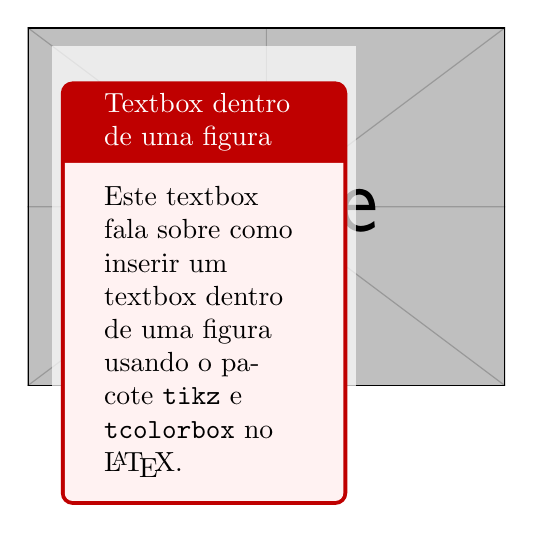
\begin{tikzpicture}
        \node[anchor=south west,inner sep=0] (image) at (0,0) {\includegraphics[width=0.5\textwidth]{example-image}}; % Substitua example-image pelo nome da sua imagem
        \begin{scope}[x={(image.south east)},y={(image.north west)}]
            % Definindo o textbox dentro da figura
            \node[anchor=north west, text width=0.3\textwidth, fill=white, opacity=0.7, text opacity=1] at (0.05,0.95) { % Ajuste a posição conforme necessário
                \begin{tcolorbox}[colback=red!5!white,colframe=red!75!black,title=Textbox dentro de uma figura]
                    Este textbox fala sobre como inserir um textbox dentro de uma figura usando o pacote \texttt{tikz} e \texttt{tcolorbox} no \LaTeX.
                \end{tcolorbox}
            };
        \end{scope}
    \end{tikzpicture}
    \caption{Figura com Textbox}
    \label{fig:figura_com_textbox1}
\end{figure}

\begin{figure}[ht]
    \centering
 \begin{tcolorbox}
Este é o conteúdo do meu textbox sem título. Você pode adicionar qualquer texto aqui, bem como incluir fórmulas matemáticas, listas e outros elementos que desejar. A caixa ajustará automaticamente o tamanho para acomodar seu conteúdo. O textbox agora foi posto dentro de uma figura.
\end{tcolorbox}
    \caption{Figura com Textbox simples}
    \label{fig:figura_com_textbox}
\end{figure}

  \chapter{Método Proposto}
  \chapter{Resultados e Discuss\~oes}

  \section{Algumas Demonstra{\c c}\~oes}

  A  Lista de Símbolos precisa usar comandos específicos. Aqui vamos usar os símbolos $\alpha$ e $\beta$.
  \symbl[beta]{Beta}{A palavra Beta more e corrigida}
  \symbl[zzbeta]{$\beta$}{A letra $\beta$ corrigida}
  \symbl{beta}{A palavra beta}
  \symbl{alpha}{A palavra alpha}
  \symbl[alpha]{Alpha}{A palavra Alpha}
  \symbl[zzalpha]{$\alpha$}{A letra $\alpha$ corrigida}
  \symbl[marco]{Marco}{A palavra Marco corrigida}

  A Lista de Abreviações segue, a partir de 2024, a mesma regra, e aqui seguem alguns exemplos.
  \abbrev{GoT}{Game of Thrones}
  \abbrev[GOT]{GoT}{Game of Thrones ordenado como GOT}
  \abbrev[iot]{IoT}{IoT ordenado como iot}
  \abbrev[IoT]{IoT}{IoT ordenado como IoT}
  \abbrev[IOT]{IoT}{IoT ordenado como IOT}
  \abbrev{IoT}{IoT com ordenação default}
  \abbrev[ITU]{ITU}{ITU mesmo}

  \chapter{Conclus\~oes}

  \backmatter
  \bibliographystyle{coppe-unsrt}
  \bibliography{example}

\appendix

\chapter{Um apêndice}

Segundo a norma da ABNT (Associação Brasileira de Normas Técnicas), a definição e utilização de apêndices e anexos seguem critérios específicos para a organização de documentos acadêmicos e técnicos.

Apêndice: O apêndice é um texto ou documento elaborado pelo autor do trabalho com o objetivo de complementar sua argumentação, sem que seja essencial para a compreensão do conteúdo principal do documento. O uso de apêndices é indicado para incluir dados detalhados como questionários, modelos de formulários utilizados na pesquisa, descrições extensas de métodos ou técnicas, entre outros. Os apêndices são identificados por letras maiúsculas consecutivas, travessão e pelos respectivos títulos. A inclusão de apêndices visa a fornecer informações adicionais que possam ajudar na compreensão do estudo, mas cuja presença no texto principal poderia distrair ou desviar a atenção do leitor dos argumentos principais.

\renewcommand{\appendixname}{Anexo}
\appendix

\chapter{Um Anexo}
Segundo a norma da ABNT (Associação Brasileira de Normas Técnicas), a definição e utilização de apêndices e anexos seguem critérios específicos para a organização de documentos acadêmicos e técnicos.

Anexo: O anexo, por sua vez, consiste em um texto ou documento não elaborado pelo autor, que serve de fundamentação, comprovação e ilustração. O uso de anexos é apropriado para materiais como cópias de artigos, legislação, documentos históricos, fotografias, mapas, entre outros, que tenham relevância para o entendimento do trabalho do autor. Assim como os apêndices, os anexos são identificados por letras maiúsculas consecutivas, travessão e pelos respectivos títulos. Eles são utilizados para enriquecer o trabalho com informações de suporte, garantindo que o leitor tenha acesso a documentos complementares importantes para a validação dos argumentos apresentados no texto principal.
\end{document}

%% 
%%
%% End of file `example.tex'.
